\documentclass{sig-alternate-2013}
% --- Author Metadata here ---
\newfont{\mycrnotice}{ptmr8t at 7pt}
\newfont{\myconfname}{ptmri8t at 7pt}
\let\crnotice\mycrnotice%
\let\confname\myconfname%

\permission{Permission to make digital or hard copies of part or all of this work for personal or classroom use is granted without fee provided that copies are not made or distributed for profit or commercial advantage and that copies bear this notice and the full citation on the first page. Copyrights for third-party components of this work must be honored. For all other uses, contact the Owner/Author(s). Copyright is held by the owner/author(s).}
\conferenceinfo{ACM DEV 2015,}{December 1--2, 2015, London, United Kingdom.} 
\copyrightetc{ACM \the\acmcopyr}
\crdata{978-1-4503-3490-7/15/11. \\
DOI: http://dx.doi.org/10.1145/2830629.2835221}
% Update the XXX's to the DOI assigned by ACM rightsreview forms

\clubpenalty=10000 
\widowpenalty = 10000
% --- End of Author Metadata --- 
% --- Image support for png ---
\usepackage{graphicx}
\graphicspath{ {images/} }
 \usepackage{url}

\begin{document}
\title{Improving Flight Accuracy for Aerial Wildlife Surveys in Sub-Saharan Africa}
% author block
\author{
Howard Frederick$^{1}$, Edward Kohi$^{2}$, Jay Lorenzo$^{3}$, Michael Coyote$^{3}$, Ted Schmitt$^{3}$ and Kirk Larsen$^{3}$\\	
\affaddr$^{1}$Independent consultant, Arusha, Tanzania; simbamangu@gmail.com \\
\affaddr$^{2}$TAWIRI, Arusha, Tanzania; edward.kohi@yahoo.co.uk  \\
\affaddr$^{3}$Vulcan, Inc, Seattle, WA; \{jayl, michaelc, teds, kirkl\}@vulcan.com
}
\maketitle

\begin{abstract}
Aerial surveys are vital to assessing animal populations as part of an effort to understand ecosystem health, a primary component of social and economic development in rural regions of Africa. This paper describes the design, deployment and preliminary performance results of a mobile application that provides visual real-time feedback to assist cockpit crews conducting aerial surveys.
\end{abstract}

% A category with the (minimum) three required fields
\category{H.5.2}{User Interfaces}{Graphical user interfaces (GUI) }
%A category including the fourth, optional field follows...
\category{J.7}{Computers In Other Systems}{Real time}

\keywords{Flight Data Logger; Transect; Aerial Survey}

\section{Introduction}
Healthy ecosystems, including thriving wildlife populations, are a major component of social and economic development across many regions in rural Africa. The monitoring of wildlife populations, including the use of aerial surveys, is essential to healthy ecosystems as it informs wildlife management planning, identifies poaching hotspots, and tracks ecological trends.

A common method of aerial survey called a systematic reconnaissance flight, or transect sample count, is conducted by flying carefully defined lines in a given region, counting the animals observed within the strips visible from each side of the aircraft and then extrapolating to estimate the total population \cite{mike}.  The lines, called transects, must be flown within a precise altitude, speed and course to minimize the extrapolation errors and to enable comparison with previous results where possible.  

Maintaining altitude and course is difficult since multiple instruments typically need to be referenced simultaneously by the pilot (e.g. altimeter, GPS and airspeed).  Consistency in flying performance is important not only for general safety but also for providing a consistent platform for observation, and minimizing biases. The software and hardware package described in this paper was designed to reduce the burden on the pilot by integrating altimeter, speed and GPS into a single console with a graphical indicator and altitude deviation.  

The software further simplifies the management of flying individual transects by allowing a flight plan of transects to be pre-loaded, as well as logging flight data automatically instead of by the manual recording on paper by a Front Seat Observer (FSO) or surveyor.  

This paper describes the design and usage of an Android-based survey assistance device we call the Flightlogger, developed as part of the Great Elephant Census project \cite{gec} (GEC), which makes improvements in these areas:

(i) \textit{Flight accuracy}. Provide an in-flight management system that helps the pilot navigate to and maintain course on individual transects through a real-time integrated display of altitude, speed and location.

(ii) \textit{Cognitive load reduction}. Automate the collection of flight data such as transect start/stops and altitude readings enabling the FSO to focus upon collecting other data.

(iii) \textit{Flight data error reduction}. Provide a pre-flight system that loads a full flight plan (e.g. transects for a given region and day) via GPX files and provide a post-flight system that downloads the recorded flight data.

Additional requirements were to create a unit with a cost below \$500 USD, that was ruggedized for rural African environments. It required intuitive UI controls to minimize the amount of training needed, and had to be easily installable in a wide variety of survey aircraft.
\section{Design and Implementation}
The Flightlogger system is based on a 7" Android tablet, which acquires altitude readings from a laser altimeter mounted externally on the survey aircraft.  The tablet is mounted to the aircraft dashboard using a small flight case containing a 3D-printed tablet mount, supplemental battery for all-day flying and a serial to USB converter which interfaces with the USB port on the tablet.

The system includes a set of distributed services that are responsible for sampling and validating incoming data from sensor and altimeter input, and assembling it into time sensitive samples. It then broadcasts that data every second for use by the logging and user facing components of the system.

One goal of this design was to allow the tablet to be detached from the system and carried by the survey team for preflight setup and post-flight analysis. During flight planning, surveyors plot the routes and transects for the survey on laptops or workstations, save the routes using the GPX interchange format, and transfer them to the tablet via USB.
The device is then reattached to the flight case, which initializes and displays a set of status lights. The purpose of these lights is to give a visual representation of altimeter, GPS and battery health. These status lights provide a means of alerting the survey team to possible issues that may arise both preflight and during the flight.  

To choose a transect to survey, the user selects from a list of routes that are displayed on the tablet. Once a route is selected, the device displays the distance to the first transect, and provides a means to start logging flight data. Data is logged every second, which relieves the FSO from manually recording altitude samples and transect waypoints. 

The flight interface mimics a standard Instrument Landing System (ILS) cockpit display, leveraging the pilot training that goes into interpreting the graphical altitude and course markers on an ILS display. When flying a specified transect, deviation from the target course is shown with one marker (vertical), while deviation from the target altitude is shown by another (horizontal; in combination the two show a crosshair). If the aircraft goes outside of the expected range (in altitude or course) then the markers change color as an additional visual cue. To increase flight accuracy, altimeter readings obtained while flying over trees and other natural features, are averaged within a 5 second window. 

\begin{figure}[h]
\centering
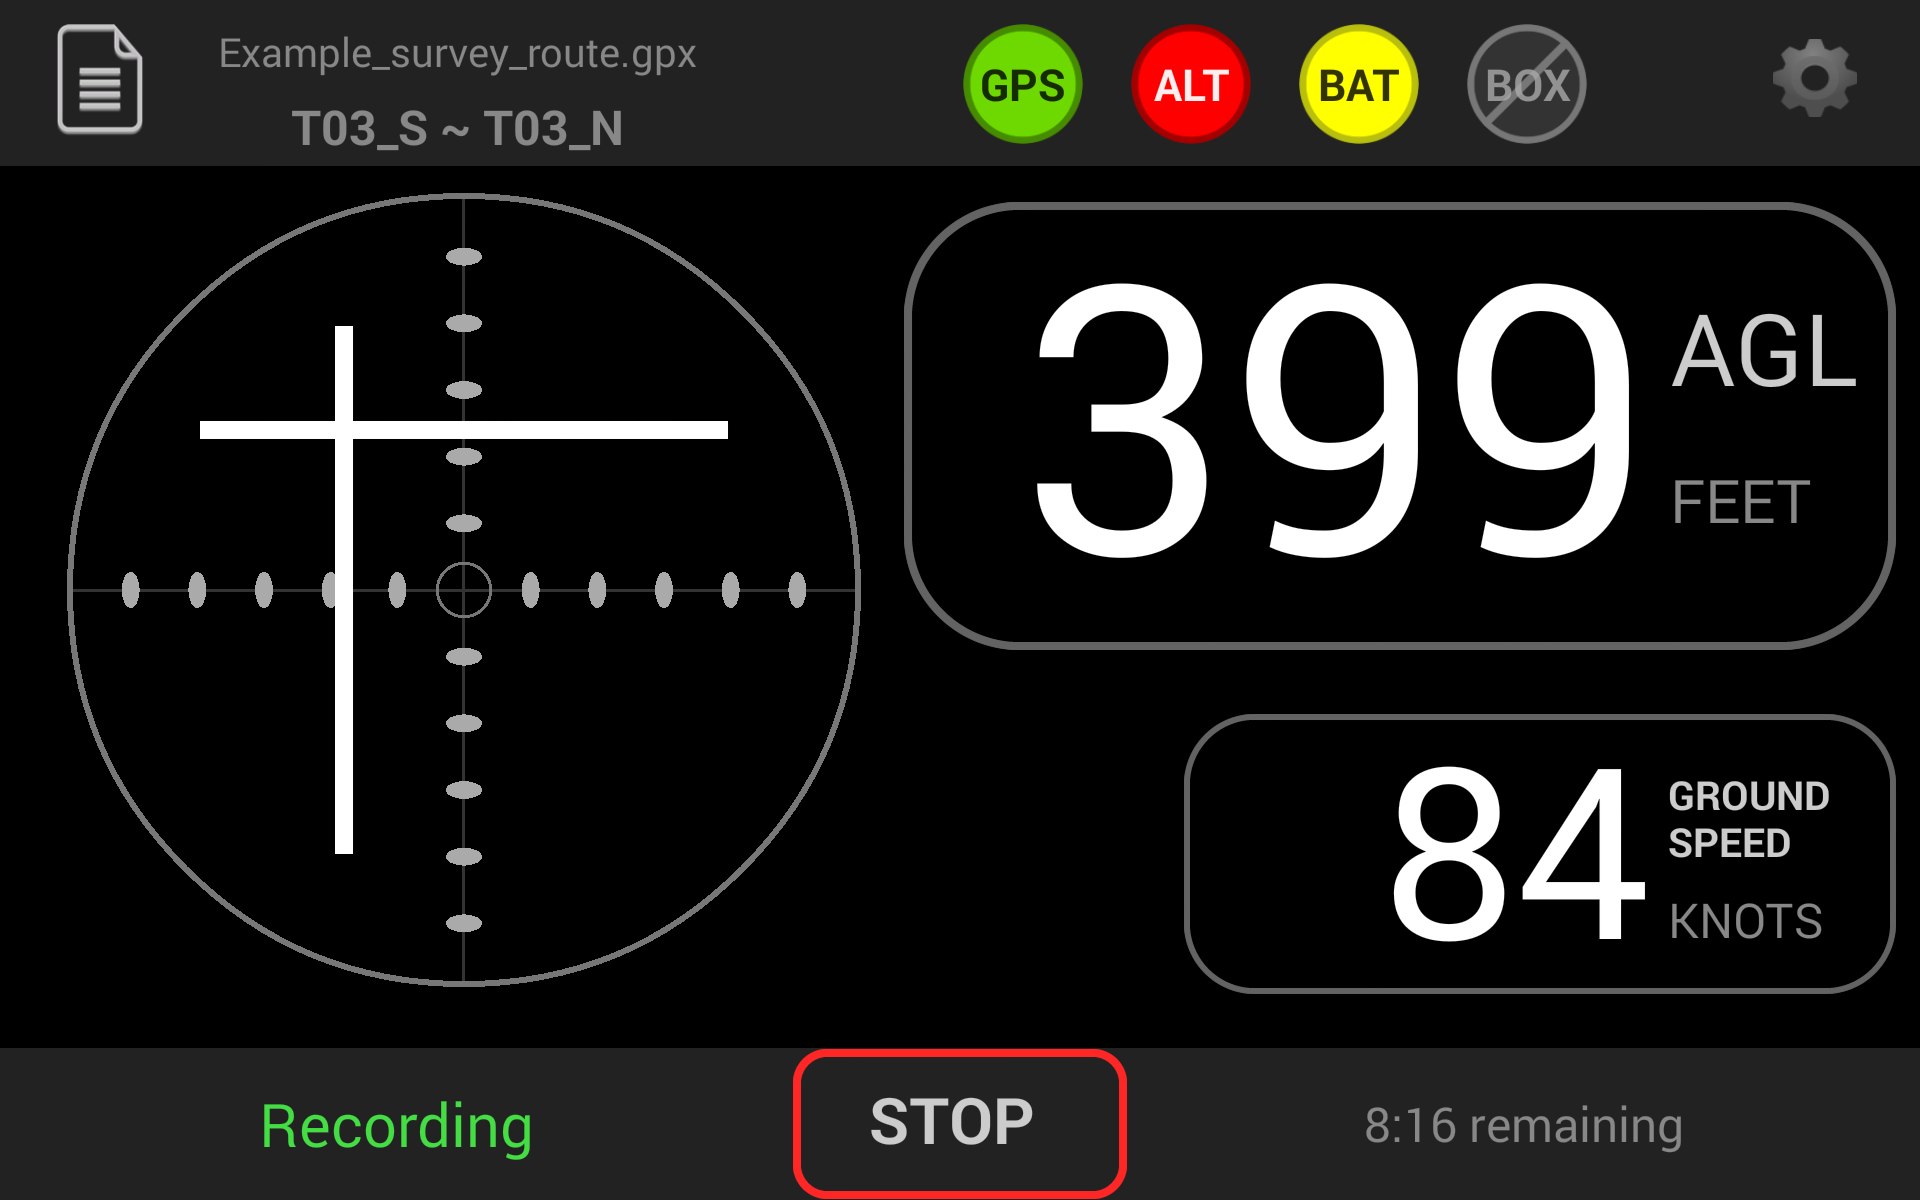
\includegraphics[width=0.9\columnwidth]{mainscreen}
\caption{Flightlogger main interface}
\end{figure}

Post flight, the tablet provides a means to summarize the transects flown, generating both GPX- and CSV-formatted reports of the data collected. The survey teams can then download the reports for further analysis by attaching the tablet to their laptop.

\section{Evaluation}
As our work has been in support of the ongoing GEC it has been difficult to obtain experimentally significant measurements of the impact of Flightlogger over the course of the census because repeat survey flights are not pragmatic. 

We have however, been able to make comparisons using similar aircraft and pilots in the field, which we believe is representative of the results that have been achieved to date.

We examine three survey flights flown in similar terrain in sub-Saharan Africa, evaluating differences between planes and pilots. We compare the deviation from desired survey height (AGL) for three flights in Figure 2.

Surveys flown with the Flightlogger display smaller deviations than those flown with a traditional radar altimeter system, and a smaller range of deviations, indicating that flight performance is improved.
\begin{figure}[h]
\centering
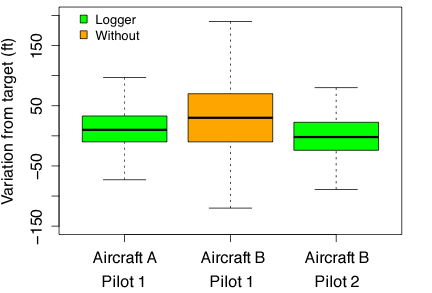
\includegraphics[width=0.9\columnwidth]{altplot13c}
\caption{Transect accuracy with and without the flight data logger, with boxplots showing deviations from target heights.}
\end{figure}

Not easily captured in statistics is the improved workflow in the cockpit, as the front seat observer is relieved of numerous data capture tasks, reducing cognitive load. 

The GEC has flown 18 of 21 countries planned to date. The Flightlogger system has been used by eight crews surveying in Kenya, Tanzania, Mozambique, Zimbabwe, Botswana, Zambia, and the Western trans boundary countries, representing a majority of overall elephant populations. 

\section{Conclusions}
The Flightogger has provided a focused technical intervention that has been shown to increase the productivity of aerial surveys supporting the GEC, at least as shown by preliminary and anecdotal results. 

Acceptance of the Flightlogger has been favorable. We initially anticipated building 10 units for the GEC, but have sent 19 to date, with further requests indicating positive adoption. 
%Teams are requesting further feature development and Tanzanian field teams are expecting to transition to using %almost exclusively this laser/logger system. 
Future work will include evaluating this project with more data and in more detail, and to look at end to end system problems of the GEC.

\section{Acknowledgements}
We are indebted to Falk Grossman and Dr. Mike Chase
for their support and feedback. We are grateful to the Paul G. Allen Family Foundation for the funding
of the Great Elephant Census. Our thanks go to the GEC PI team at Vulcan, especially Dr. Kathleen Gobush, Lauren Kickham and Joel Masselink.

\bibliographystyle{acm}
\bibliography{flightlogger}


\end{document}
